\documentclass[12pt,a4paper]{article}
\usepackage{amsmath,amsthm,amssymb,mathtools}
\usepackage{tikz}
\usetikzlibrary{arrows.meta,positioning,shapes.geometric,calc,fit,backgrounds}
\usepackage{graphicx}
\usepackage{booktabs,tabularx,multirow}
\usepackage[ruled,vlined,linesnumbered]{algorithm2e}
\usepackage[most]{tcolorbox}
\usepackage{hyperref}
\usepackage[capitalize,noabbrev]{cleveref}
\usepackage[margin=1in]{geometry}
\usepackage{fancyhdr}
\usepackage{enumitem}
\usepackage{xcolor}
\newtcolorbox{keyinsight}[1][]{colback=blue!5!white,colframe=blue!75!black,fonttitle=\bfseries,title=Key Insight,#1}
\newtcolorbox{example}[1][]{colback=green!5!white,colframe=green!75!black,fonttitle=\bfseries,title=Example,#1}
\newtcolorbox{warningbox}[1][]{colback=red!5!white,colframe=red!75!black,fonttitle=\bfseries,title=Warning,#1}
\newtheorem{theorem}{Theorem}[section]
\newtheorem{lemma}[theorem]{Lemma}
\newtheorem{definition}{Definition}[section]
\newtheorem{remark}{Remark}[section]

% -----------------------------------------------------------
% Header / Footer
% -----------------------------------------------------------
\pagestyle{fancy}
\fancyhf{}
\rhead{Deep Learning -- Session 22}
\lhead{Seq2Seq Architecture \& Limitations}
\rfoot{\thepage}
\lfoot{IIITDwd, February 2026}

% -----------------------------------------------------------
% Metadata
% -----------------------------------------------------------
\title{%
  \vspace{-1cm}
  \Large\textbf{Deep Learning Course}\\[0.4em]
  \huge\textbf{Session 22: Sequence-to-Sequence Architecture and Its Limitations}\\[0.6em]
  \large Encoder--Decoder Models, Autoregressive Decoding, and the Context-Vector Bottleneck
}
\author{%
  Prof.\ S R M Prasanna \and Dr.\ Sunil Saumya\\[0.2em]
  \normalsize Indian Institute of Information Technology, Dharwad (IIITDwd)
}
\date{February 7, 2026 \quad (Deck: \texttt{10-Seq2Seq}, 25 slides)}

% ============================================================
\begin{document}
% ============================================================

\maketitle
\thispagestyle{fancy}

\begin{abstract}
This document is a comprehensive set of notes for Session~22 of the Deep Learning course at IIITDwd.
The session covers the motivation for sequence-to-sequence (Seq2Seq) models, the encoder--decoder
architecture built on LSTM units, the autoregressive inference procedure (teacher forcing vs.\ greedy
decoding), and the critical limitations that arise from compressing an entire source sequence into a
single fixed-size context vector. The final part of the session presents a hands-on PyTorch
implementation of Seq2Seq for English-to-Hindi machine translation.
These limitations directly motivate the attention mechanism introduced in Session~24.
\end{abstract}

\tableofcontents
\newpage

% ============================================================
\section{Introduction}
\label{sec:introduction}
% ============================================================

By Session~22, the course has covered three principal neural-network families:
\begin{itemize}[noitemsep]
  \item \textbf{Fully-connected (ANN)} -- suitable for tabular, fixed-length, order-independent inputs.
  \item \textbf{Convolutional (CNN)} -- designed for spatially structured data such as images; exploits
        local correlations and weight sharing.
  \item \textbf{Recurrent (RNN / LSTM / GRU)} -- tailored for sequential data where temporal ordering
        matters; maintains a hidden state that evolves over time steps.
\end{itemize}

Each family was motivated by a concrete data modality and a shortcoming of its predecessor. This
session introduces a \emph{fourth} paradigm: the \textbf{sequence-to-sequence (Seq2Seq)} model. The
central problem is that all three families above map an input of a fixed structure to an output of a
fixed structure. Real applications such as machine translation, text summarisation, and question
answering, however, require \emph{variable-length input $\to$ variable-length output} mappings -- a
regime none of the preceding architectures handles naturally.

\begin{keyinsight}
  The fundamental mismatch that Seq2Seq solves: a source sentence of length $T_x$ must be
  mapped to a target sentence of length $T_y$, where $T_x$ and $T_y$ are \emph{independent}
  and unknown at model-design time. Neither vanilla RNNs nor LSTMs provide a direct mechanism
  for this ``many-to-many with mismatched lengths'' setting.
\end{keyinsight}

The historical context is also important: the Seq2Seq architecture was proposed in 2014 in the
landmark paper ``Sequence to Sequence Learning with Neural Networks'' by Sutskever, Vinyals, and
Le~\cite{sutskever2014}. It used multi-layer LSTMs for both the encoder and decoder and achieved
state-of-the-art results on English-to-French translation at the time.

% ============================================================
\section{Background: Recap of Sequential Models}
\label{sec:background}
% ============================================================

\subsection{Vanilla RNN Limitations}

A vanilla RNN processes a sequence $\mathbf{x} = (x_1, x_2, \ldots, x_T)$ by updating a hidden
state:
\begin{equation}
  h_t = \tanh\!\left(W_{hh}\,h_{t-1} + W_{xh}\,x_t + b_h\right),
  \label{eq:rnn_hidden}
\end{equation}
where $W_{hh}$ and $W_{xh}$ are shared weight matrices. The output at each step is
$\hat{y}_t = \text{softmax}(W_{hy}\,h_t + b_y)$. Because gradients must backpropagate through
many time steps, vanilla RNNs suffer from the vanishing/exploding gradient problem and cannot
reliably capture long-range dependencies.

\subsection{LSTM: Gated Memory}

The Long Short-Term Memory (LSTM) cell addresses this by introducing explicit gating:
\begin{align}
  f_t &= \sigma\!\left(W_f [h_{t-1}, x_t] + b_f\right) & &\text{(forget gate)} \label{eq:lstm_f}\\
  i_t &= \sigma\!\left(W_i [h_{t-1}, x_t] + b_i\right) & &\text{(input gate)} \label{eq:lstm_i}\\
  \tilde{C}_t &= \tanh\!\left(W_C [h_{t-1}, x_t] + b_C\right) & &\text{(candidate cell)} \label{eq:lstm_cc}\\
  C_t &= f_t \odot C_{t-1} + i_t \odot \tilde{C}_t & &\text{(cell state update)} \label{eq:lstm_c}\\
  o_t &= \sigma\!\left(W_o [h_{t-1}, x_t] + b_o\right) & &\text{(output gate)} \label{eq:lstm_o}\\
  h_t &= o_t \odot \tanh(C_t) & &\text{(hidden state)} \label{eq:lstm_h}
\end{align}
The LSTM maintains \emph{two} memory tensors: the cell state $C_t$ (long-term memory) and the
hidden state $h_t$ (short-term / working memory). This dual-memory design allows relevant
information to persist over hundreds of time steps.

\subsection{GRU: Lighter Alternative}

The Gated Recurrent Unit (GRU) merges the two memory tensors into a single hidden state, using only
a reset gate $r_t$ and an update gate $z_t$:
\begin{align}
  r_t &= \sigma\!\left(W_r [h_{t-1}, x_t]\right), \label{eq:gru_r}\\
  z_t &= \sigma\!\left(W_z [h_{t-1}, x_t]\right), \label{eq:gru_z}\\
  \tilde{h}_t &= \tanh\!\left(W [r_t \odot h_{t-1}, x_t]\right), \label{eq:gru_htilde}\\
  h_t &= (1 - z_t) \odot h_{t-1} + z_t \odot \tilde{h}_t. \label{eq:gru_h}
\end{align}

\begin{keyinsight}
  LSTM vs.\ GRU: both architectures handle long-range dependencies comparably in practice.
  The GRU has fewer parameters (three gates vs.\ four) and typically trains faster. The choice
  between them should be made empirically: run both, compare validation accuracy, and prefer the
  lighter GRU if performance is equivalent.
\end{keyinsight}

\subsection{Comparison of Sequential Models}

\begin{table}[htbp]
  \centering
  \caption{Comparison of sequential neural-network variants.}
  \label{tab:rnn_comparison}
  \begin{tabular}{@{}lcccc@{}}
    \toprule
    \textbf{Model} & \textbf{Memory type} & \textbf{Gates} & \textbf{Params (hidden $d$)} & \textbf{Long-range capability} \\
    \midrule
    Vanilla RNN & Single $h_t$ & 0 & $\mathcal{O}(d^2)$ & Poor \\
    LSTM        & $h_t$ + $C_t$  & 4 & $\mathcal{O}(4d^2)$ & Good \\
    GRU         & Single $h_t$ & 3 & $\mathcal{O}(3d^2)$ & Good \\
    \bottomrule
  \end{tabular}
\end{table}

% ============================================================
\section{Seq2Seq Motivation}
\label{sec:motivation}
% ============================================================

\subsection{The Variable-Length Mapping Problem}

Consider English-to-Hindi translation:
\begin{center}
  \textit{``I am going''} $\;\longrightarrow\;$ \textit{``main ja raha hoon''}
\end{center}
The source has 3 tokens; the target has 4 tokens. More importantly, the correspondence is
\emph{non-monotonic}: ``going'' maps to two words (``ja raha''), and the subject ``I'' (``main'')
appears last in the Hindi sentence. A standard RNN that produces one output per input time step
cannot handle this.

\begin{example}[title={Why word-by-word translation fails}]
  Suppose we naively apply an LSTM in a one-to-one fashion, producing one Hindi token per English
  token:
  \[
    \underbrace{I}_{\text{step 1}} \to \underbrace{\text{main}}_{\hat{y}_1}, \quad
    \underbrace{\text{am}}_{\text{step 2}} \to \underbrace{?}_{\hat{y}_2}, \quad
    \underbrace{\text{going}}_{\text{step 3}} \to \underbrace{?}_{\hat{y}_3}.
  \]
  Problems: (i) ``going'' requires two Hindi words; (ii) word order differs; (iii) the model cannot
  produce the correct output for step~2 without knowing the full sentence meaning first.
  Hence word-by-word translation is fundamentally incorrect.
\end{example}

\subsection{Use Cases Requiring Seq2Seq}

\begin{table}[htbp]
  \centering
  \caption{Applications of Seq2Seq models with typical input/output length relationships.}
  \label{tab:usecases}
  \begin{tabular}{@{}llcc@{}}
    \toprule
    \textbf{Task} & \textbf{Description} & \textbf{Input length} & \textbf{Output length} \\
    \midrule
    Machine Translation & Source $\to$ target language & Variable & Different variable \\
    Text Summarisation  & Paragraph $\to$ summary      & Long ($\sim$50 words) & Short ($\sim$10 words) \\
    Question Answering  & Question + context $\to$ answer & Long & Short \\
    Speech Recognition  & Audio frames $\to$ text tokens & Very long & Short \\
    Code Generation     & Natural language $\to$ code snippet & Medium & Medium \\
    \bottomrule
  \end{tabular}
\end{table}

The key insight: the correct approach is to \emph{first encode the entire source sequence into a
compact representation}, and \emph{then decode that representation} into the target sequence one
token at a time. This encoder--decoder split is the central innovation of Seq2Seq models.

% ============================================================
\section{Encoder--Decoder Architecture}
\label{sec:architecture}
% ============================================================

\subsection{Overview}

The Seq2Seq model consists of two components:
\begin{enumerate}[noitemsep]
  \item \textbf{Encoder} -- reads the source sequence and produces a \emph{context vector}.
  \item \textbf{Decoder} -- initialised with the context vector, generates the target sequence
        token by token.
\end{enumerate}

\begin{definition}[Context Vector]
  \label{def:context_vector}
  The \emph{context vector} $\mathbf{c}$ is the final hidden state (and, for LSTM, the cell
  state) of the encoder after processing the entire source sequence:
  \[
    \mathbf{c} = \bigl(h_{T_x}^{(\text{enc})},\; C_{T_x}^{(\text{enc})}\bigr).
  \]
  It is a fixed-dimensional vector that is intended to encode the \emph{meaning} of the source
  sequence in its entirety.
\end{definition}

\subsection{TikZ Diagram: Encoder--Decoder Architecture}
\label{subsec:enc_dec_diagram}

\begin{figure}[htbp]
  \centering
  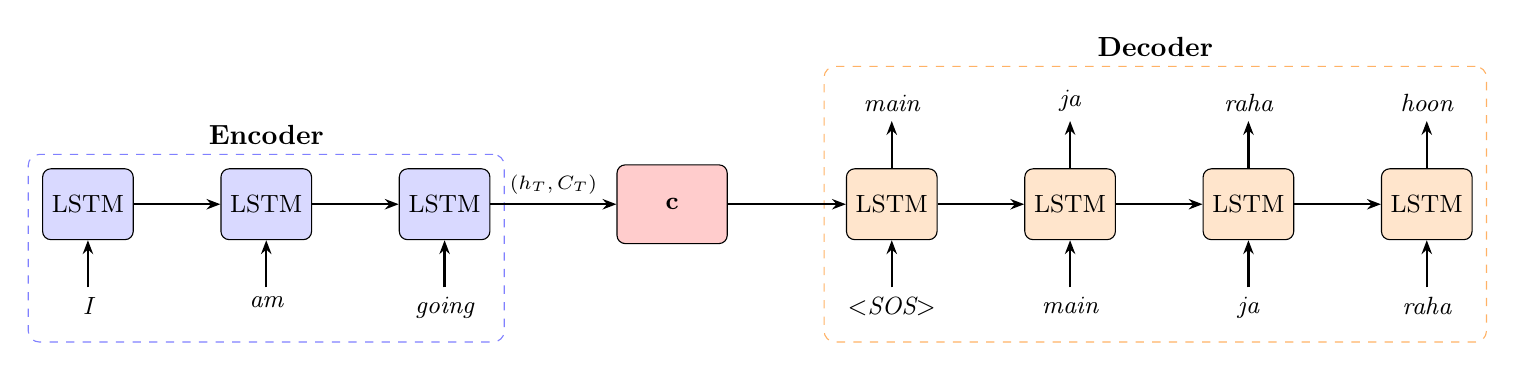
\begin{tikzpicture}[
      node distance=0.9cm and 1.1cm,
      lstm/.style={draw, rectangle, minimum width=1.1cm, minimum height=0.9cm,
                   fill=blue!15, rounded corners=3pt, font=\small},
      dlstm/.style={draw, rectangle, minimum width=1.1cm, minimum height=0.9cm,
                    fill=orange!20, rounded corners=3pt, font=\small},
      token/.style={font=\small\itshape},
      arrow/.style={-{Stealth[length=5pt]}, thick},
      cvec/.style={draw, rectangle, minimum width=1.4cm, minimum height=1.0cm,
                   fill=red!20, rounded corners=3pt, font=\small\bfseries},
    ]
    % ---- Encoder ----
    \node[lstm] (e1) {LSTM};
    \node[lstm, right=of e1] (e2) {LSTM};
    \node[lstm, right=of e2] (e3) {LSTM};

    % encoder inputs
    \node[token, below=0.6cm of e1] (w1) {I};
    \node[token, below=0.6cm of e2] (w2) {am};
    \node[token, below=0.6cm of e3] (w3) {going};

    % encoder arrows
    \draw[arrow] (w1) -- (e1);
    \draw[arrow] (w2) -- (e2);
    \draw[arrow] (w3) -- (e3);
    \draw[arrow] (e1) -- (e2);
    \draw[arrow] (e2) -- (e3);

    % context vector
    \node[cvec, right=1.6cm of e3] (cv) {$\mathbf{c}$};
    \draw[arrow] (e3) -- node[above, font=\scriptsize]{$(h_T, C_T)$} (cv);

    % ---- Decoder ----
    \node[dlstm, right=1.5cm of cv] (d1) {LSTM};
    \node[dlstm, right=of d1] (d2) {LSTM};
    \node[dlstm, right=of d2] (d3) {LSTM};
    \node[dlstm, right=of d3] (d4) {LSTM};

    % decoder inputs (bottom)
    \node[token, below=0.6cm of d1] (s0) {\textless{}SOS\textgreater};
    \node[token, below=0.6cm of d2] (t1d) {main};
    \node[token, below=0.6cm of d3] (t2d) {ja};
    \node[token, below=0.6cm of d4] (t3d) {raha};

    % decoder inputs from below
    \draw[arrow] (s0) -- (d1);
    \draw[arrow] (t1d) -- (d2);
    \draw[arrow] (t2d) -- (d3);
    \draw[arrow] (t3d) -- (d4);

    % decoder hidden connections
    \draw[arrow] (d1) -- (d2);
    \draw[arrow] (d2) -- (d3);
    \draw[arrow] (d3) -- (d4);

    % context vector to decoder init
    \draw[arrow] (cv) -- (d1);

    % decoder outputs (top)
    \node[token, above=0.6cm of d1] (o1) {main};
    \node[token, above=0.6cm of d2] (o2) {ja};
    \node[token, above=0.6cm of d3] (o3) {raha};
    \node[token, above=0.6cm of d4] (o4) {hoon};

    \draw[arrow] (d1) -- (o1);
    \draw[arrow] (d2) -- (o2);
    \draw[arrow] (d3) -- (o3);
    \draw[arrow] (d4) -- (o4);

    % bounding boxes
    \begin{scope}[on background layer]
      \node[draw=blue!50, dashed, rounded corners, fit=(e1)(e2)(e3)(w1)(w2)(w3),
            label=above:{\textbf{Encoder}}, inner sep=5pt] {};
      \node[draw=orange!60, dashed, rounded corners,
            fit=(d1)(d2)(d3)(d4)(s0)(t1d)(t2d)(t3d)(o1)(o2)(o3)(o4),
            label=above:{\textbf{Decoder}}, inner sep=5pt] {};
    \end{scope}
  \end{tikzpicture}
  \caption{Seq2Seq encoder--decoder architecture for English-to-Hindi translation.
           The encoder produces a context vector $\mathbf{c}=(h_T, C_T)$ that initialises
           the decoder. During training, teacher forcing supplies the true target tokens as
           decoder inputs; at inference, the previous prediction is fed back.}
  \label{fig:enc_dec}
\end{figure}

\subsection{Encoder Forward Pass}

Let the source sequence be $\mathbf{x} = (x_1, x_2, \ldots, x_{T_x})$. The encoder is an
$L$-layer LSTM. At each time step $t$:
\begin{align}
  \mathbf{e}_t &= E_{\text{src}}\,x_t, \label{eq:src_embed}\\
  (h_t^{(\text{enc})}, C_t^{(\text{enc})}) &= \text{LSTM}_{\text{enc}}\!\left(\mathbf{e}_t,\; h_{t-1}^{(\text{enc})},\; C_{t-1}^{(\text{enc})}\right), \label{eq:enc_step}
\end{align}
where $E_{\text{src}} \in \mathbb{R}^{d_e \times |V_{\text{src}}|}$ is the source embedding matrix.
After processing the full source, the context vector is:
\begin{equation}
  \mathbf{c} = \bigl(h_{T_x}^{(\text{enc})},\; C_{T_x}^{(\text{enc})}\bigr).
  \label{eq:context_vec}
\end{equation}

\subsection{Decoder Forward Pass}

The decoder is also an LSTM, initialised with $\mathbf{c}$. At time step $t$:
\begin{align}
  \mathbf{e}'_t &= E_{\text{tgt}}\,y_{t-1}, \label{eq:tgt_embed}\\
  (h_t^{(\text{dec})}, C_t^{(\text{dec})}) &= \text{LSTM}_{\text{dec}}\!\left(\mathbf{e}'_t,\; h_{t-1}^{(\text{dec})},\; C_{t-1}^{(\text{dec})}\right), \label{eq:dec_step}\\
  \hat{y}_t &= \text{softmax}\!\left(W_{\text{out}}\,h_t^{(\text{dec})} + b_{\text{out}}\right), \label{eq:dec_output}
\end{align}
where $y_0 = \langle\text{SOS}\rangle$ is the start-of-sequence token.

\begin{keyinsight}
  The encoder's final state $(h_{T_x}, C_{T_x})$ directly initialises the decoder's initial
  state $(h_0^{(\text{dec})}, C_0^{(\text{dec})})$. This is why the LSTM's dual-memory design
  (hidden state + cell state) is especially natural for Seq2Seq: both tensors carry complementary
  information about the encoded source.
\end{keyinsight}

% ============================================================
\section{Training: Teacher Forcing}
\label{sec:training}
% ============================================================

\subsection{Loss Function}

Training is supervised. Each example is a pair $(\mathbf{x}, \mathbf{y})$ where $\mathbf{y} =
(y_1, y_2, \ldots, y_{T_y})$ is the ground-truth target sequence. The loss is cross-entropy
summed over all decoding steps:
\begin{equation}
  \mathcal{L} = -\sum_{t=1}^{T_y} \log P\!\left(y_t \mid y_1, \ldots, y_{t-1}, \mathbf{x}\right)
              = -\sum_{t=1}^{T_y} \log \hat{y}_t[y_t],
  \label{eq:seq2seq_loss}
\end{equation}
where $\hat{y}_t[y_t]$ denotes the predicted probability of the true token $y_t$.

\subsection{Teacher Forcing}

During training, the true target token $y_{t-1}$ is fed as the decoder input at step $t$,
regardless of what the model predicted at step $t-1$. This strategy is called \textbf{teacher
forcing}:
\begin{equation}
  \text{(training)}\qquad \text{decoder input at step }t = y_{t-1}^{(\text{true})}.
  \label{eq:teacher_forcing}
\end{equation}

\begin{example}[title={Teacher Forcing for ``I am going'' $\to$ ``main ja raha hoon''}]
  Decoder steps during training:
  \begin{center}
    \begin{tabular}{@{}cccc@{}}
      \toprule
      Step $t$ & Decoder input & Predicted $\hat{y}_t$ & Ground truth $y_t$ \\
      \midrule
      1 & \textless{}SOS\textgreater & main & main \\
      2 & main (true) & ja & ja \\
      3 & ja (true) & raha & raha \\
      4 & raha (true) & hoon & hoon \\
      5 & hoon (true) & \textless{}EOS\textgreater & \textless{}EOS\textgreater \\
      \bottomrule
    \end{tabular}
  \end{center}
  At each step, the \emph{true} previous token is supplied, not the model's prediction.
  This stabilises training but creates a train--test distribution mismatch.
\end{example}

\begin{warningbox}
  \textbf{Exposure Bias:} Teacher forcing uses ground-truth tokens during training, but at
  inference the model must use its \emph{own predictions}. If the model makes an error at
  step $t$, that erroneous token is fed as input at step $t+1$, potentially compounding
  errors throughout the sequence. This train--inference gap is called \emph{exposure bias}
  and remains an active research topic (scheduled sampling, REINFORCE, etc.).
\end{warningbox}

% ============================================================
\section{Inference: Autoregressive Decoding}
\label{sec:inference}
% ============================================================

\subsection{Greedy Decoding}

At inference time, no ground-truth labels are available. The decoder operates
\emph{autoregressively}: each generated token is fed back as the input for the next step:
\begin{equation}
  y_t = \arg\max_{v \in V} P\!\left(v \mid y_1, \ldots, y_{t-1}, \mathbf{x}\right)
      = \arg\max_v \hat{y}_t[v],
  \label{eq:greedy}
\end{equation}
with $y_0 = \langle\text{SOS}\rangle$. Generation continues until the model produces
$\langle\text{EOS}\rangle$ or a maximum length is reached. Compactly:
\begin{equation}
  y_t = \text{Decoder}\!\left(y_{t-1},\; \mathbf{c}\right).
  \label{eq:autoregressive}
\end{equation}

\subsection{TikZ Diagram: Autoregressive Inference}
\label{subsec:autoregressive_diagram}

\begin{figure}[htbp]
  \centering
  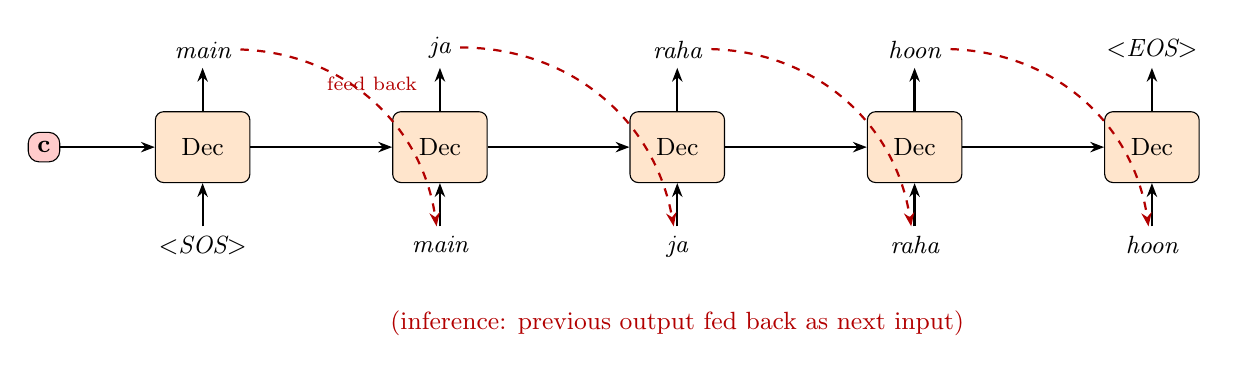
\begin{tikzpicture}[
      node distance=0.7cm and 1.2cm,
      lstm/.style={draw, rectangle, minimum width=1.2cm, minimum height=0.9cm,
                   fill=orange!20, rounded corners=3pt, font=\small},
      tok/.style={font=\small\itshape},
      arrow/.style={-{Stealth[length=5pt]}, thick},
      feedback/.style={-{Stealth[length=5pt]}, thick, dashed, bend left=40, color=red!70!black},
    ]

    \node[lstm] (d0) {Dec};
    \node[lstm, right=1.8cm of d0] (d1) {Dec};
    \node[lstm, right=1.8cm of d1] (d2) {Dec};
    \node[lstm, right=1.8cm of d2] (d3) {Dec};
    \node[lstm, right=1.8cm of d3] (d4) {Dec};

    % inputs from below
    \node[tok, below=0.55cm of d0] (i0) {\textless{}SOS\textgreater};
    \node[tok, below=0.55cm of d1] (i1) {main};
    \node[tok, below=0.55cm of d2] (i2) {ja};
    \node[tok, below=0.55cm of d3] (i3) {raha};
    \node[tok, below=0.55cm of d4] (i4) {hoon};

    % outputs above
    \node[tok, above=0.55cm of d0] (o0) {main};
    \node[tok, above=0.55cm of d1] (o1) {ja};
    \node[tok, above=0.55cm of d2] (o2) {raha};
    \node[tok, above=0.55cm of d3] (o3) {hoon};
    \node[tok, above=0.55cm of d4] (o4) {\textless{}EOS\textgreater};

    % vertical arrows
    \draw[arrow] (i0) -- (d0);
    \draw[arrow] (i1) -- (d1);
    \draw[arrow] (i2) -- (d2);
    \draw[arrow] (i3) -- (d3);
    \draw[arrow] (i4) -- (d4);

    \draw[arrow] (d0) -- (o0);
    \draw[arrow] (d1) -- (o1);
    \draw[arrow] (d2) -- (o2);
    \draw[arrow] (d3) -- (o3);
    \draw[arrow] (d4) -- (o4);

    % horizontal hidden connections
    \draw[arrow] (d0) -- (d1);
    \draw[arrow] (d1) -- (d2);
    \draw[arrow] (d2) -- (d3);
    \draw[arrow] (d3) -- (d4);

    % feedback arrows
    \draw[feedback] (o0) to node[above, font=\scriptsize\color{red!70!black}]{feed back} (i1);
    \draw[feedback] (o1) to (i2);
    \draw[feedback] (o2) to (i3);
    \draw[feedback] (o3) to (i4);

    % context vector entering d0
    \node[draw, fill=red!20, rounded corners, left=1.2cm of d0, font=\small\bfseries] (cv) {$\mathbf{c}$};
    \draw[arrow] (cv) -- (d0);

    % label
    \node[below=1.5cm of d2, font=\small\color{red!70!black}]
      {(inference: previous output fed back as next input)};
  \end{tikzpicture}
  \caption{Autoregressive decoding at inference time. The dashed red arrows show the feedback
           loop: the predicted token at step $t$ becomes the input at step $t+1$. The context
           vector $\mathbf{c}$ initialises the first decoder cell.}
  \label{fig:autoregressive}
\end{figure}

\subsection{Algorithm: Seq2Seq Inference}

\begin{algorithm}[H]
  \caption{Seq2Seq Greedy Decoding}
  \label{alg:seq2seq_inference}
  \KwIn{Source sequence $\mathbf{x} = (x_1, \ldots, x_{T_x})$; trained encoder and decoder;
        vocabulary $V$; maximum target length $T_{\max}$}
  \KwOut{Generated target sequence $\hat{\mathbf{y}}$}

  \BlankLine
  \tcp{Step 1: Encode source}
  $h_0^{(\text{enc})} \leftarrow \mathbf{0}$, $C_0^{(\text{enc})} \leftarrow \mathbf{0}$\;
  \For{$t \leftarrow 1$ \KwTo $T_x$}{
    $\mathbf{e}_t \leftarrow E_{\text{src}}\,x_t$\;
    $(h_t^{(\text{enc})}, C_t^{(\text{enc})}) \leftarrow \text{LSTM}_{\text{enc}}(\mathbf{e}_t,\, h_{t-1}^{(\text{enc})},\, C_{t-1}^{(\text{enc})})$\;
  }
  $\mathbf{c} \leftarrow (h_{T_x}^{(\text{enc})},\, C_{T_x}^{(\text{enc})})$\;

  \BlankLine
  \tcp{Step 2: Decode autoregressively}
  $h_0^{(\text{dec})} \leftarrow h_{T_x}^{(\text{enc})}$, $C_0^{(\text{dec})} \leftarrow C_{T_x}^{(\text{enc})}$\;
  $y_0 \leftarrow \langle\text{SOS}\rangle$\;
  $\hat{\mathbf{y}} \leftarrow [\;]$\;
  \For{$t \leftarrow 1$ \KwTo $T_{\max}$}{
    $\mathbf{e}'_t \leftarrow E_{\text{tgt}}\,y_{t-1}$\;
    $(h_t^{(\text{dec})}, C_t^{(\text{dec})}) \leftarrow \text{LSTM}_{\text{dec}}(\mathbf{e}'_t,\, h_{t-1}^{(\text{dec})},\, C_{t-1}^{(\text{dec})})$\;
    $\hat{y}_t \leftarrow \text{softmax}(W_{\text{out}}\,h_t^{(\text{dec})} + b_{\text{out}})$\;
    $y_t \leftarrow \arg\max_{v \in V}\;\hat{y}_t[v]$\;
    $\hat{\mathbf{y}} \leftarrow \hat{\mathbf{y}} \cup [y_t]$\;
    \If{$y_t = \langle\text{EOS}\rangle$}{\textbf{break}\;}
  }
  \Return $\hat{\mathbf{y}}$\;
\end{algorithm}

% ============================================================
\section{Limitations: The Context-Vector Bottleneck}
\label{sec:limitations}
% ============================================================

\subsection{The Bottleneck Problem}

Despite its elegance, the Seq2Seq architecture has a fundamental limitation: \textbf{all
information from the source sequence must be compressed into a single, fixed-dimensional
context vector $\mathbf{c}$}.

For short sentences this is manageable. For long sentences, the LSTM must fit an arbitrarily
long sequence of information into a vector of fixed size $d$. This creates two distinct failure
modes, one on each side of the architecture.

\begin{keyinsight}
  The context-vector bottleneck is not a failure of LSTM design but an architectural
  constraint imposed by the encoder--decoder split. No matter how large $d$ is, information
  \emph{must} be compressed. The attention mechanism, introduced in Session~24, addresses this
  by giving the decoder access to \emph{all} encoder hidden states rather than just the final
  one.
\end{keyinsight}

\subsection{Encoder-Side Problem}

When the source sentence is long, the LSTM encoder must simultaneously retain information about
early tokens and late tokens within the same fixed-size cell state $C_{T_x}$. Because gates
are applied multiplicatively:
\begin{equation}
  C_t = f_t \odot C_{t-1} + i_t \odot \tilde{C}_t,
  \label{eq:cell_overwrite}
\end{equation}
later inputs have a tendency to ``overwrite'' earlier content whenever $f_t$ is small. For a
sentence of $T_x$ tokens, the contribution of token $x_1$ to the final $C_{T_x}$ is
approximately:
\begin{equation}
  \left(\prod_{k=2}^{T_x} f_k\right) C_0 \approx 0 \quad \text{for large } T_x.
  \label{eq:forget_product}
\end{equation}
This means early words in a long source sentence tend to be forgotten by the time the encoder
finishes.

\subsection{Decoder-Side Problem}

The decoder uses \emph{the same} context vector $\mathbf{c}$ at every decoding step. There is
no mechanism for the decoder to focus on different parts of the source at different generation
steps. For example, when generating the first Hindi word the decoder ideally needs information
about the subject; when generating the verb it needs information about the verb in the source.
But $\mathbf{c}$ is static -- it cannot adapt.

\begin{remark}
  This decoder-side limitation is qualitatively different from the encoder-side one. Even if the
  encoder perfectly compressed all source information into $\mathbf{c}$, the decoder still cannot
  selectively retrieve \emph{relevant} parts of that information at each step, because
  $\mathbf{c}$ is a single undifferentiated vector.
\end{remark}

\subsection{Quantitative Summary of Limitations}

\begin{table}[htbp]
  \centering
  \caption{Summary of Seq2Seq limitations and their consequences.}
  \label{tab:limitations}
  \begin{tabular}{@{}p{3cm}p{5.5cm}p{5cm}@{}}
    \toprule
    \textbf{Location} & \textbf{Problem} & \textbf{Consequence} \\
    \midrule
    Encoder & Long sequences cannot be fully compressed into $\mathbf{c}$ & Early tokens are forgotten; quality degrades rapidly with source length \\
    \midrule
    Decoder & Same $\mathbf{c}$ used at every generation step & No dynamic focus; decoder cannot attend to relevant source tokens per step \\
    \midrule
    Both & Fixed-size bottleneck regardless of sequence complexity & Translation quality plateaus and then drops for long sentences \\
    \bottomrule
  \end{tabular}
\end{table}

\subsection{Empirical Evidence}

It was shown empirically (Cho et al., 2014~\cite{cho2014}) that BLEU scores of basic Seq2Seq
models degrade sharply once source sentences exceed roughly 20--30 words. This motivated
Bahdanau et al.\ (2015)~\cite{bahdanau2015} to introduce the attention mechanism, which
replaces the single fixed context vector with a \emph{dynamic weighted sum} over all encoder
hidden states.

% ============================================================
\section{Hands-On Implementation: PyTorch Seq2Seq}
\label{sec:implementation}
% ============================================================

\subsection{Data Preparation}

For the machine translation demo, a small English-to-Hindi corpus is used. Each example is a
pair $(\mathbf{x}_{\text{src}}, \mathbf{y}_{\text{tgt}})$ of tokenised sentences. The
vocabulary is built by iterating over all training sentences, and words are mapped to integer
indices. Special tokens are:
\begin{itemize}[noitemsep]
  \item \texttt{<PAD>} (index 0) -- padding to equalise batch lengths.
  \item \texttt{<SOS>} (index 1) -- start-of-sequence token prepended to every target.
  \item \texttt{<EOS>} (index 2) -- end-of-sequence token appended to every target.
  \item \texttt{<UNK>} (index 3) -- out-of-vocabulary words.
\end{itemize}

\subsection{Encoder Module}

The encoder wraps an \texttt{nn.Embedding} layer followed by an \texttt{nn.LSTM}:

\begin{tcolorbox}[colback=gray!5!white,colframe=gray!60!black,title=\texttt{Encoder} (PyTorch)]
\begin{verbatim}
class Encoder(nn.Module):
    def __init__(self, input_size, embedding_dim,
                 hidden_size, num_layers):
        super().__init__()
        self.embedding = nn.Embedding(input_size,
                                      embedding_dim)
        self.rnn = nn.LSTM(embedding_dim, hidden_size,
                           num_layers=num_layers,
                           batch_first=True)

    def forward(self, x):
        # x: [batch, src_len]
        embedded = self.embedding(x)
        # embedded: [batch, src_len, emb_dim]
        outputs, (hidden, cell) = self.rnn(embedded)
        # hidden: [num_layers, batch, hidden_size]
        # cell:   [num_layers, batch, hidden_size]
        return hidden, cell
\end{verbatim}
\end{tcolorbox}

Note that \texttt{outputs} (all encoder hidden states) are discarded in the basic Seq2Seq model;
only the final \texttt{(hidden, cell)} pair is used as the context vector. This is exactly
where the bottleneck arises -- all intermediate states are thrown away.

\subsection{Decoder Module}

\begin{tcolorbox}[colback=gray!5!white,colframe=gray!60!black,title=\texttt{Decoder} (PyTorch)]
\begin{verbatim}
class Decoder(nn.Module):
    def __init__(self, output_size, embedding_dim,
                 hidden_size, num_layers):
        super().__init__()
        self.embedding = nn.Embedding(output_size,
                                      embedding_dim)
        self.rnn = nn.LSTM(embedding_dim, hidden_size,
                           num_layers=num_layers,
                           batch_first=True)
        self.fc = nn.Linear(hidden_size, output_size)

    def forward(self, x, hidden, cell):
        # x: [batch] (single token per step)
        x = x.unsqueeze(1)           # [batch, 1]
        embedded = self.embedding(x) # [batch, 1, emb]
        output, (hidden, cell) = self.rnn(
            embedded, (hidden, cell))
        # output: [batch, 1, hidden_size]
        pred = self.fc(output.squeeze(1))
        # pred: [batch, output_size]
        return pred, hidden, cell
\end{verbatim}
\end{tcolorbox}

\subsection{Seq2Seq Wrapper}

\begin{tcolorbox}[colback=gray!5!white,colframe=gray!60!black,title=\texttt{Seq2Seq} (PyTorch)]
\begin{verbatim}
class Seq2Seq(nn.Module):
    def __init__(self, encoder, decoder, device):
        super().__init__()
        self.encoder = encoder
        self.decoder = decoder
        self.device  = device

    def forward(self, src, tgt,
                teacher_forcing_ratio=0.5):
        batch_size = src.shape[0]
        tgt_len    = tgt.shape[1]
        tgt_vocab  = self.decoder.fc.out_features
        outputs    = torch.zeros(batch_size,
                                 tgt_len,
                                 tgt_vocab
                                ).to(self.device)
        hidden, cell = self.encoder(src)
        x = tgt[:, 0]  # <SOS>
        for t in range(1, tgt_len):
            out, hidden, cell = \
                self.decoder(x, hidden, cell)
            outputs[:, t] = out
            teacher = random.random() < \
                          teacher_forcing_ratio
            x = tgt[:, t] if teacher \
                           else out.argmax(1)
        return outputs
\end{verbatim}
\end{tcolorbox}

\subsection{Sanity Check}

After instantiating the encoder, a quick check verifies that tensor shapes are correct:

\begin{tcolorbox}[colback=gray!5!white,colframe=gray!60!black,title=Shape Sanity Check]
\begin{verbatim}
for src_batch, tgt_batch in train_loader:
    e_h, e_c = encoder(src_batch)
    print("e_h shape:", e_h.shape)
    # Expected: [num_layers, batch_size, hidden_size]
    print("e_c shape:", e_c.shape)
    # Expected: [num_layers, batch_size, hidden_size]
    break
\end{verbatim}
\end{tcolorbox}

The shapes confirm that both the hidden state and cell state for all LSTM layers are captured in
the context vector.

\subsection{Training Loop Sketch}

Training uses cross-entropy loss ignoring padding tokens:
\begin{equation}
  \mathcal{L}_{\text{batch}} = \frac{1}{N\,T_y}
    \sum_{n=1}^{N}\sum_{t=1}^{T_y}
    \mathbf{1}[y_{n,t} \neq \text{PAD}]\cdot
    \left(-\log \hat{y}_{n,t}[y_{n,t}]\right),
  \label{eq:masked_loss}
\end{equation}
where $N$ is the batch size. The \texttt{ignore\_index} argument of
\texttt{nn.CrossEntropyLoss} handles the masking automatically.

% ============================================================
\section{Towards Attention: Motivating Session 24}
\label{sec:towards_attention}
% ============================================================

The bottleneck identified in \cref{sec:limitations} motivates a natural question: instead of
forcing the decoder to use a single static $\mathbf{c}$, why not let it access \emph{all}
encoder hidden states $(h_1^{(\text{enc})}, \ldots, h_{T_x}^{(\text{enc})})$ and compute a
\emph{dynamic, step-dependent} context?

This is precisely the attention mechanism. At each decoder step $t$, an attention score
$\alpha_{t,s}$ is computed for each encoder position $s$:
\begin{equation}
  \alpha_{t,s} = \frac{\exp(e_{t,s})}{\sum_{s'=1}^{T_x}\exp(e_{t,s'})},
  \quad e_{t,s} = \text{score}\!\left(h_t^{(\text{dec})},\, h_s^{(\text{enc})}\right),
  \label{eq:attention}
\end{equation}
and the dynamic context vector is:
\begin{equation}
  \mathbf{c}_t = \sum_{s=1}^{T_x} \alpha_{t,s}\,h_s^{(\text{enc})}.
  \label{eq:dynamic_context}
\end{equation}

\begin{example}[title={Attention in translation}]
  When decoding the Hindi verb ``ja'' from the English ``I am going'', the attention mechanism
  would ideally assign high weight to the encoder hidden state corresponding to ``going''
  ($\alpha_{t,3}$ large) and low weight to ``I'' and ``am''. This dynamic focus is impossible
  with a static context vector.
\end{example}

% ============================================================
\section{Session Summary}
\label{sec:summary}
% ============================================================

\subsection{Key Takeaways}

This session introduced the Seq2Seq encoder--decoder architecture and its LSTM-based
implementation. The main points are:

\begin{enumerate}[noitemsep]
  \item \textbf{Motivation:} Standard ANN/CNN/RNN models cannot map variable-length sequences
        to variable-length sequences. Seq2Seq addresses this with a two-phase encoder--decoder
        pipeline (proposed in 2014).

  \item \textbf{Encoder:} An LSTM reads the entire source sequence and produces a
        \emph{context vector} $(h_{T_x}, C_{T_x})$ summarising its meaning.

  \item \textbf{Decoder:} An LSTM initialised with the context vector generates the target
        sequence one token at a time via an \emph{autoregressive} process.

  \item \textbf{Training vs.\ Inference:} During training, \emph{teacher forcing} supplies
        true target tokens as decoder inputs. During inference, the model's own predictions
        are fed back, creating potential exposure bias.

  \item \textbf{Bottleneck Limitation:} Compressing an arbitrary-length source into a
        fixed-size context vector causes information loss for long sequences. The decoder
        also cannot focus on relevant source positions per step.

  \item \textbf{Motivation for Attention:} The bottleneck is resolved by providing the decoder
        with access to all encoder hidden states weighted by a learned attention distribution
        (Session~24).
\end{enumerate}

\subsection{Mathematical Notation Reference}

\begin{table}[htbp]
  \centering
  \caption{Summary of mathematical notation used in this session.}
  \label{tab:notation}
  \begin{tabular}{@{}cll@{}}
    \toprule
    \textbf{Symbol} & \textbf{Meaning} & \textbf{Dimensions} \\
    \midrule
    $h_t^{(\text{enc})}$ & Encoder hidden state at step $t$ & $\mathbb{R}^{d_h}$ \\
    $C_t^{(\text{enc})}$ & Encoder cell state at step $t$ & $\mathbb{R}^{d_h}$ \\
    $\mathbf{c}$         & Context vector (final encoder state) & $\mathbb{R}^{d_h} \times \mathbb{R}^{d_h}$ \\
    $h_t^{(\text{dec})}$ & Decoder hidden state at step $t$ & $\mathbb{R}^{d_h}$ \\
    $\hat{y}_t$          & Predicted output distribution at step $t$ & $\mathbb{R}^{|V_{\text{tgt}}|}$ \\
    $y_t$                & Predicted (or ground-truth) token at step $t$ & $\{1, \ldots, |V_{\text{tgt}}|\}$ \\
    $T_x$                & Source sequence length & -- \\
    $T_y$                & Target sequence length & -- \\
    $d_e$                & Embedding dimension & -- \\
    $d_h$                & LSTM hidden size & -- \\
    \bottomrule
  \end{tabular}
\end{table}

% ============================================================
\section{Extended Discussion: Beam Search and Evaluation}
\label{sec:beam_search}
% ============================================================

\subsection{Greedy Decoding vs.\ Beam Search}

Greedy decoding (\cref{alg:seq2seq_inference}) is fast but suboptimal: selecting the locally
best token at each step does not guarantee the globally best sequence. \textbf{Beam search}
maintains a set of $B$ candidate hypotheses (the ``beam'') and expands each by all possible
next tokens, keeping only the top-$B$ by cumulative log-probability:
\begin{equation}
  \text{score}(\mathbf{y}_{1:t}) = \sum_{k=1}^{t} \log P(y_k \mid y_1, \ldots, y_{k-1}, \mathbf{x}).
  \label{eq:beam_score}
\end{equation}
To prevent the score from favouring shorter sequences, a length penalty is often applied:
\begin{equation}
  \text{score}_{\text{norm}}(\mathbf{y}) = \frac{\text{score}(\mathbf{y})}{T_y^\alpha},
  \quad \alpha \in (0, 1].
  \label{eq:length_penalty}
\end{equation}
Typical values are $B \in \{4, 5, 10\}$ and $\alpha \approx 0.6$--$0.7$.

\subsection{BLEU Score}

The standard automatic metric for machine translation is the
\textbf{Bilingual Evaluation Understudy (BLEU)} score~\cite{papineni2002}.
BLEU measures $n$-gram precision between the hypothesis $\hat{\mathbf{y}}$ and one or more
reference translations $\mathbf{y}^{(r)}$:
\begin{equation}
  \text{BLEU} = \text{BP} \cdot \exp\!\left(\sum_{n=1}^{N} w_n \log p_n\right),
  \label{eq:bleu}
\end{equation}
where $p_n$ is the clipped $n$-gram precision, $w_n = 1/N$ (uniform weights for $N=4$), and
$\text{BP}$ is the brevity penalty:
\begin{equation}
  \text{BP} = \begin{cases} 1 & \text{if } |\hat{\mathbf{y}}| > |\mathbf{y}^{(r)}|, \\
                            e^{1 - |\mathbf{y}^{(r)}|/|\hat{\mathbf{y}}|} & \text{otherwise.}
              \end{cases}
  \label{eq:bp}
\end{equation}

\begin{warningbox}[title={BLEU Limitations}]
  BLEU is a proxy metric. It does not capture semantic adequacy, fluency beyond $n$-gram
  overlap, or handling of morphologically rich languages. Modern evaluation increasingly
  uses neural metrics such as BERTScore or ChrF, alongside human evaluation.
\end{warningbox}

% ============================================================
\section{Frequently Asked Questions from Session 22}
\label{sec:faq}
% ============================================================

The following questions arose during the live class session and are reproduced with expanded
answers.

\begin{description}[style=nextline, leftmargin=0pt]

  \item[Q: When should we use LSTM vs.\ GRU?]
    Both LSTM and GRU handle long-range dependencies comparably. The main practical difference
    is model complexity: GRU has approximately $3d^2$ parameters per layer vs.\ $4d^2$ for LSTM
    (where $d$ is the hidden size). Use GRU when training speed or model size is a constraint;
    use LSTM when you suspect the extra gating capacity may help. Always validate empirically on
    your specific task and dataset -- do not assume one is universally better.

  \item[Q: Is the context vector a single tensor or two tensors?]
    For LSTM, the context vector consists of \emph{two} tensors: the hidden state $h_{T_x}$ and
    the cell state $C_{T_x}$. Both are passed to initialise the decoder. In PyTorch, the LSTM
    returns \texttt{(hidden, cell)}, each of shape
    \texttt{[num\_layers, batch\_size, hidden\_size]}. When people informally refer to ``the
    context vector'' as a single entity, they mean this pair collectively.

  \item[Q: Why does the decoder input need a \textless{}SOS\textgreater{} token?]
    The LSTM always requires both a sequence-token input and a previous hidden state. At the
    first decoder step ($t=1$), there is no previous predicted token, so a sentinel token
    \textless{}SOS\textgreater{} is used to signal ``start decoding now.'' Its embedding is
    learnable and is effectively a ``boot'' signal for the decoder.

  \item[Q: Does the same context vector appear at every decoder step?]
    In the basic Seq2Seq model: yes. The context vector $\mathbf{c} = (h_{T_x}, C_{T_x})$ is
    used \emph{only} to initialise the decoder state at $t=0$. Thereafter, the decoder evolves
    its own hidden state. The context vector does not re-appear explicitly at steps $t > 1$.
    (Some variants concatenate $\mathbf{c}$ to every decoder input, but the original Sutskever
    et al.\ paper only uses it for initialisation.)

\end{description}

% ============================================================
% References
% ============================================================
\begin{thebibliography}{9}

\bibitem{sutskever2014}
Sutskever, I., Vinyals, O., and Le, Q.\ V. (2014).
\textit{Sequence to Sequence Learning with Neural Networks.}
Advances in Neural Information Processing Systems (NeurIPS), 27.

\bibitem{cho2014}
Cho, K., van Merri\"{e}nboer, B., Gulcehre, C., Bahdanau, D., Bougares, F.,
Schwenk, H., and Bengio, Y. (2014).
\textit{Learning Phrase Representations using RNN Encoder--Decoder for Statistical Machine Translation.}
EMNLP 2014.

\bibitem{bahdanau2015}
Bahdanau, D., Cho, K., and Bengio, Y. (2015).
\textit{Neural Machine Translation by Jointly Learning to Align and Translate.}
ICLR 2015.

\bibitem{hochreiter1997}
Hochreiter, S.\ and Schmidhuber, J. (1997).
\textit{Long Short-Term Memory.}
Neural Computation, 9(8), 1735--1780.

\bibitem{chung2014}
Chung, J., Gulcehre, C., Cho, K., and Bengio, Y. (2014).
\textit{Empirical Evaluation of Gated Recurrent Neural Networks on Sequence Modeling.}
NIPS 2014 Workshop.

\bibitem{papineni2002}
Papineni, K., Roukos, S., Ward, T., and Zhu, W.-J. (2002).
\textit{BLEU: a Method for Automatic Evaluation of Machine Translation.}
ACL 2002, pp.\ 311--318.

\bibitem{williams1989}
Williams, R.\ J.\ and Zipser, D. (1989).
\textit{A Learning Algorithm for Continually Running Fully Recurrent Neural Networks.}
Neural Computation, 1(2), 270--280.

\end{thebibliography}

\end{document}
